\section*{Введение}
\addcontentsline{toc}{section}{Введение}

По мере развития цифровых микросхем возникло противоречие между возможной
степенью интеграции и номенклатурой выпускаемых микросхем. Экономически
оправдано было выпускать микросхемы средней интеграции, таких как регистры,
счетчики, сумматоры. Более сложные схемы приходилось создавать из этих узлов.
Разместить более сложную схему на полупроводниковом кристалле не было проблем,
но это было оправдано либо очень большой серийностью аппаратуры, либо ценой
аппаратуры (военная, авиационная или космическая). Заказные микросхемы не могли
удовлетворить возникшую потребность в миниатюризации аппаратуры. Решение могло
быть только одним -- предоставить разработчикам аппаратуры возможность изменять
внутреннюю структуру микросхемы (программировать).

История развития программируемых логических интегральных схем (ПЛИС) начинается
с появления программируемых постоянных запоминающих устройств. Первое время
программируемые ПЗУ использовались исключительно для хранения данных, однако
вскоре их стали применять для реализации цифровых комбинаторных устройств с
произвольной таблицей истинности. В качестве недостатка подобного решения
следует отметить экспоненциальный рост сложности устройства в зависимости от
количества входов. Добавление одного дополнительного входа цифрового устройства
приводит к удвоению требуемого количества ячеек памяти ПЗУ. Это не позволяет
реализовать многовходовые комбинационные цифровые схемы. 

\vspace*{2em} % ----------------------------------------------------------------

\section{Что такое ПЛИС. Области его применения}

ПЛИС (программируемая логическая интегральная схема) -- это большие
интегральные микросхемы матричного типа, позволяющие программным способом
реализовать логические функции большой сложности. Физическим ограничением
быстродействия присущей всем традиционным архитектурам процессоров является
последовательное выполнение команд. Всевозможные ухищрения вроде
суперскалярности, мультиконвейерности, многоядерности не сильно скрашивают эту
картину. Архитектура ПЛИС имеют потенциально большее быстродействие по
сравнению с микроконтроллерами и DSP процессорами. Это объясняется возможностью
аппаратного распараллеливания вычислений.


Основные области применения ПЛИС:
\begin{itemize}
    \item высокоскоростная обработка данных;
    \item алгоритмы ЦОС, особенно где требуется обработка данных в реальном
    времени;
    \item задачи обработки информации, требующие большого количества
    пользовательских выводов;
    \item промежуточных этап проектирования СБИС;
    \item узкоспециальные алгоритмы, построенные на жестких временных
    диаграммах;
    \item проекты, где требуется большое число портов ввода-вывода.
\end{itemize}

\vspace*{2em} % ----------------------------------------------------------------

\section{Классификация ПЛИС}

 Классификация программируемых логических интегральных схем
приведена на рисунке \ref{pic_1}.
\begin{figure}[h!]
    \centering
    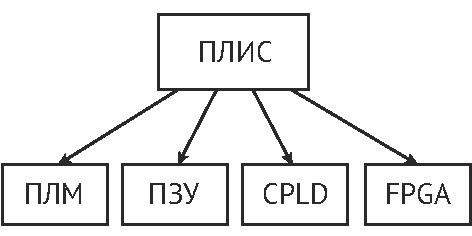
\includegraphics[width=.6\textwidth]{pld_01}
    \caption{Классификация программируемых логических интегральных схем (ПЛИС)}
    \label{pic_1}
\end{figure}

Программируемые логические матрицы (ПЛМ) реализуют хорошо известные принципы
создания цифровой комбинационной схемы по таблице истинности (СДНФ). Применение
постоянных запоминающих устройств (ПЗУ) в качестве комбинационной схемы
позволяет вообще обойтись без составления комбинационной функции и ее
минимизации.

В настоящее время наибольшую распространенность получили два типа архитектур
ПЛИС:
\begin{enumerate}
    \item CPLD (англ. \emph{Complex Programmable Logic Device}). Примерами ПЛИС
    данной архитектуры является семейство MAX фирмы Altera и CoolRunner фирмы
    Xilinx. Для архитектур данных ПЛИС характерны крупные логические блоки --
    макроячейки (macrocells). Современные ПЛИС содержат до нескольких сотен
    макроячеек. Каждая макроячейка реализует функцию нескольких переменных и
    содержит триггер для хранения полученного результата. Для ПЛИС данной
    архитектуры характерно крайне низкая потребляемая мощность в статическом
    режиме (потребляемый ток порядка десятков микроампер), которая линейно
    возрастает с увеличением тактовой частоты. Также для данной архитектуры
    характерны жесткие временные задержки между макроячейками, а следовательно
    и выводами микросхемы. Типичное время задержки между выводами (pin-to-pin)
    составляет единицы наносекунд. Прошивка ПЛИС данной архитектуры хранится
    внутри микросхемы в энергонезависимой памяти.
    
    \item FPGA (англ. \emph{Field-Programmable Gate Array}). ПЛИС данной
    архитектуры обладают намного более развитой архитектурой, по сравнению с
    CPLD. Основной структурной единицей ПЛИС данной архитектуры является LUT
    (англ. \emph{LookUp Tables}) -- таблицы преобразования, позволяющие
    реализовывать логические функции. Современные ПЛИС содержат аппаратные
    умножители, в том числе с накоплением (MAC), блоки внутренней памяти,
    аппаратные интерфейсы для DDRx SDRAM, аппаратные ядра PCIexpress,
    встроенные микропроцессорные ядра, трансиверы для организации скоростной
    передачи данных между ПЛИС и внешними устройствами.
\end{enumerate}

В процессе проектирования устройств на ПЛИС используют языки описания устройств
HDL (\emph{Hardware Description Language}) -- VHDL, Verilog, Abel, AHDL. Ранее
был распространен способ проектирования с помощью рисования схемотехники. Этап
проектирования устройства на ПЛИС заключается в описании устройства на языке
HDL, перевода описания в базис выбранной ПЛИС, трассировка внутренних ресурсов
ПЛИС в соответствии со списком цепей, генерация результирующей прошивки.

\vspace*{2em} % ----------------------------------------------------------------

\section{Простейшие ПЛИС - программируемые логические матрицы (ПЛМ)}

Программируемые логические матрицы -- наиболее традиционный тип ПЛИС, имеющий
программируемые матрицы ``И'' и ``ИЛИ''. В зарубежной литературе
соответствующими этому классу аббревиатурами являются FPLA (\emph{Field
Programmable Logic Array}) и FPLS (\emph{Field Programmable Logic Sequensers}).
Примерами таких ПЛИС могут служить отечественные схемы K556PT1, PT2, PT21.

Построение ПЛМ основано на том, что любая комбинационная функция может быть
представлена в виде логической суммы (операция ИЛИ) логических произведений
(операций И). Тогда схема реализующая комбинационную функцию может быть
представлена в виде, показанном на рисунке \ref{pic_2}.
\begin{figure}[h!]
    \centering
    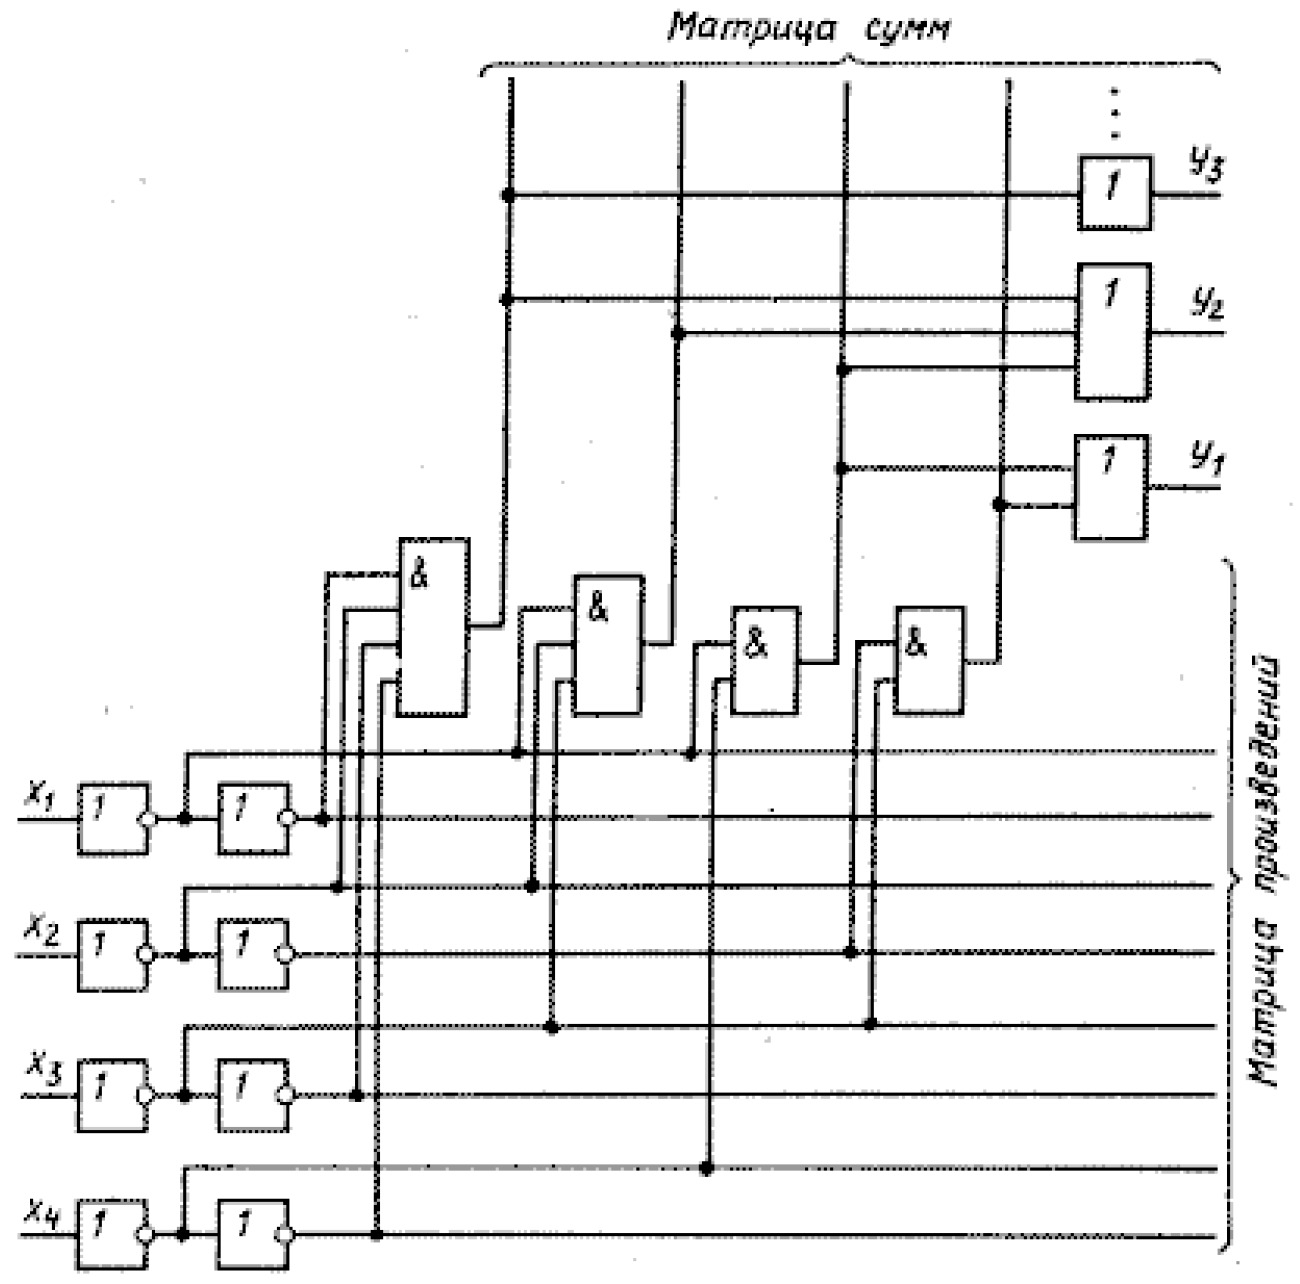
\includegraphics[width=.6\textwidth]{pld_02}
    \caption{Представление комбинационной функции}
    \label{pic_2}
\end{figure}

Недостаток такой архитектуры -- слабое использование ресурсов программируемой
матрицы ``ИЛИ'', поэтому дальнейшее развитие получили микросхемы, построенные
по архитектуре программируемой матричной логики (PAL - \emph{Programmable Array
Logic}) - это ПЛИС, имеющие программируемую матрицу ``И'' и фиксированную
матрицу ``ИЛИ''. К этому классу относятся большинство современных ПЛИС
небольшой степени интеграции.  Разновидностью этого класса
являются ПЛИС, имеющие только одну (программируемую) матрицу ``И'', например,
схема 85C508 фирмы INTEL. Следующий традиционный тип ПЛИС -- программируемая
макрологика. Они содержат единственную программируемую матрицу ``И-НЕ'' или
``ИЛИ-НЕ'', но за счёт многочисленных инверсных обратных связей способны
формировать сложные логические функции. 

Вышеперечисленные архитектуры ПЛИС содержат небольшое число ячеек, к настоящему
времени морально устарели и применяются для реализации относительно простых
устройств, для которых не существует готовых ИС средней степени интеграции.
Естественно, для реализации алгоритмов ЦОС они непригодны.

\vspace*{2em} % ----------------------------------------------------------------

\section{Особенности программирования ПЛИС}

В настоящее время используются две технологии для
хранения информации о конфигурации -- статическое ОЗУ (SRAM) или электрически
перепрограммируемое ПЗУ (EPRM или EEPROM или FLASH).

При работе в подобных системах конфигурация схемы, которая должна быть получена
``внутри'' ПЛИС или алгоритм ее работы задается либо на текстовом языке
описаний (ADHL, VDHL или Verilog) напоминающем язык программирования высокого
уровня (например, Си), либо на графическом уровне -- в виде электрической схемы
(в форматах OrCAD или PCAD), либо при помощи блок-схем алгоритмов или графиков
входных и выходных сигналов. В дальнейшем все этапы работы, включая
программирование или загрузку ПЛИС выполняет автоматизированная система.

\vspace*{2em} % ----------------------------------------------------------------

\section*{Заключение}
\addcontentsline{toc}{section}{Заключение}

Стремительные преобразования такие, как количественные (увеличение плотности
ячеек на кристалле), множество качественных (разработка новых архитектур) и
принципиально новых подходов (SoC) прошедшие в производстве ПЛИС за
сравнительно короткое время дают повод полагать, что, с одной стороны, вновь
выпускаемые ИС получат более высокие технические показатели, с другой --
предлагаемые решения более низкой ценовой категории будут занимать все больше
места в приложениях, где до сегодняшнего дня использовались традиционные
методы: ИС стандартной логики и БИС.

\vspace*{2em} % ----------------------------------------------------------------
\renewcommand{\bibname}{Список источников}

\begin{thebibliography}{9} \addcontentsline{toc}{section}{Список источников}
    \bibitem{1} \href{http://de.ifmo.ru/bk_netra/page.php?tutindex=25&index=43}
    {http://de.ifmo.ru/bk\_netra/page.php?tutindex=25\&index=43}
    \bibitem{2} \href{http://www.chipovod.ru/category/plis/}
    {http://www.chipovod.ru/category/plis/}
    \bibitem{3} \href{http://digteh.ru/digital/PLD/}
    {http://digteh.ru/digital/PLD/}
\end{thebibliography}